\documentclass{article}
\usepackage[utf8]{inputenc}
\usepackage[english, polish]{babel}
\usepackage{forloop}
\usepackage[T1]{fontenc}
\usepackage{amsfonts}
\usepackage{tikz}
\usepackage{graphicx}
\usepackage{amsmath}
\usepackage{graphicx}
\newtheorem{theorem}{Theorem}[section]
\newtheorem{corollary}{Corollary}[theorem]
\newtheorem{lemma}[theorem]{Lemma}
\title{Lista 11}
\author{Łukasz Magnuszewski}
\date{\vspace{-5ex}}
%\date{} 
\begin{document}



\maketitle



\section*{Zadanie 12}
Pokazmy z twierdzenia Ore'a że jest to graf hamiltonowski.

Ustalmy dowolne $x, y \in V(G)$ takie że $\{x, y\} \not\in E(G)$. Teraz każdy z pozostałych $n-2$ wierzchołków jest połączony zarówny z x jak i y. Udowdnijmy to szybko. Ustalmy dowolne v. Z założeń zadania. Przynajmniej 3 krawędzię z następującego zbioru są w grafie. $\{ \{x,y\}, \{x,v\}, \{y,v\} \}$. Ale wiemy że x i y nie są połączone. Więc v jest połączone z x i y. Co oznacza że \[deg(x) = deg(y) = n - 2 \]. 
\[deg(x) + deg(y) = n + n - 4 > n\]. Czyli twierdzenie Ore'a zachodzi dla n > 3.


\section*{Zadanie 8}
Przyjmijmy następujące oznaczenie $A_a = \{ b \in G : \{a, b\} \in E(G) \}$

Niech $n = max \{out(v) : v \in G \}$ wtedy $\exists x \in G : out(x) = n$. Pokażmy teraz że z wierzchołka x można dojśc do każdego innego maksymalnie w dwóch krokach.

Ustalmy dowolny $v \in G : v \neq x$, 

Wiemy że $|A_x| = n$ oraz że $|A_v| \leq n$. W takim razie $n+1 = |A_x \cup \{x\}| > n \geq |A_v|$ Czyli $\exists z \in A_x \cup \{x\} : z \not\in A_v$, w takim razie jako że nie ma krawędzi z v do z, to istnieje krawędź z do v. I mamy ścieżke od długości 2:  $x \to z \to v$ (Albo 1 jeśli $x = z$). Czyli $d(x,v) \leq 2$.


\section*{Zadanie 10}

\subsection*{Droga hamiltona}
Tutaj jest przykładowa droga skoczka po szachownicy:


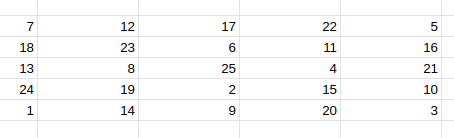
\includegraphics{skoczek}
\subsection*{Cykl hamiltona}
Zauważmy że jak potrakujemy szachownicę jako graf, którego wierzchołkami są pola szachownicy, a krawędzią są połączone te pola między którymi można się przemieścić skoczkiem w jednym ruchu. To będzie to graf dwudzielny: czarne pola to jeden podzbiór wierzchołków, zaś białe to drugi. 

Kolor pola można wyznaczyć wzorem $color(x,y) = (x+y) \mod 2$. Zaś skoczek w swoim ruchu zmienia jedną współrzędną o 2, a drugą o 1. Czyli w takim razie zmienia parzystość sumy swoich współrzędnych. Co oznacza że zmienia kolor pola na którym stoi. I rzeczywiście jest to graf dwudzielny.

W grafie dwudzielnym mogą istnieć tylko parzyste cykle. A cykl po 25 wierzchołkach ma długość 25, czyli nieparzystą. Co oznacza że nie może on istnieć.

\section*{Zadanie 9}
Indukcja po liczbie wierzchołków w grafie
\subsection*{Pooooooosadzka indukcyjna (n=1)}
Śmigaaaaaaa
\subsection*{Suuuuus indukcjny $(n-1 \implies n)$}
Jak z naszego grafu o n wierzchołkach usuniemy 1 wierzchołkach, to otrzymamy graf o $n-1$ wierzchołkach który wciąż jest turniejem, więc z założenia indukcyjnego jest w nim droga hamiltona. Teraz rozpatrzmy 3 przypadki:

Ten wierzchołek który usunęliśmy ma łuk do niego od wszystkich pozostałych wierzchołków, wtedy dostawiamy go na koniec drogi hamiltona (dla grafu n-1). 

Ten wierzchołek który usunęliśmy ma łuk z niego do wszystkich pozostałych wierzchołków, wtedy dostawiamy go na początek drogi hamiltona (dla grafu n-1). 

W pozostałych przypadkach wklejamy go po najdalszym wierzchołku w drodze hamiltona (dla grafu n-1), z którego wychodzi łuk do niego. 

Na jeden z tych trzech sposobów otrzymaliśmy drogę hamiltona dla naszego grafu o n wierzchołkach. Co kończy krok indukcyjny

\section*{Zadanie 7}
Pytanie po przetrawieniu historyjki sprowadza się do odpowiedzenia na pytanie, dla jakich n-ów W grafie $K_n$ istnieje cykl eulera. Klika jest grafem spójnym więc by istniał cykl eulera wystarczy by każdy wierzchołek miał parzysty stopień. W  klice każdy wierzchołek ma stopień równy $n-1$. Czyli by stopień każdego był parzysty n musi być nieparzyste.

\section*{Zadanie 15}
Rozważmy graf Z który powstaje przez dodanie do grafu G nowego wierzchołka który jest połączony z wszystkimi pozostałymi. Wtedy w grafie Z zachodzi \[\forall u,v \in V(Z): deg_Z(u) + deg_Z(v) = deg(u) + 1 + deg(v) + 1 \geq   n(Z) = n(G) - 1 + 1\]
Czyli z twierdzenie Ore'a w grafie Z jest cykl hamiltona. Usuwając z niego nowy wierzchołek, otrzymujemy drogę hamiltona w grafie G.

\end{document}